%============================Used packages==============================%
%-----------------------------------------------------------------------%
\documentclass[12pt]{report}
\usepackage{sagetex}
\usepackage{amsmath}

\usepackage{fancyheadings}
\pagestyle{fancy}



\usepackage{geometry}
\usepackage{graphicx}	
\usepackage[print,panelright,paneltoc]{pdfscreen}
\geometry{a4paper, margin=1.5in,
 top=1.5in,
 bottom=1in}


%-----------------------------------------------------------------------%
%==============================Labels====================================%
%------------------------------------------------------------------------%
\newcommand{\gen}[1]
{
	[#1_{{ij}}]
}
\newcommand{\eref}[1]{
	Eq.\ref{#1}
}
%-----------------------------------------------------------------------------%
%=======================Title page============================================%
%-----------------------------------------------------------------------------%
\title{Matrix Algebra: Revision}
\author{Amarjeet singh and Avi kaur}
\begin{document}
\thispagestyle{plain}
	\begin{titlepage}
\maketitle
	\end{titlepage}
%----------------------------------------------------------------------------%
%===============Chapter & variable Declaration==============================%
%----------------------------------------------------------------------------%
	\chapter{Matrix}
	\section{Introduction}
	\begin{sagesilent}
		m=var('m')
		n=var('n')
	\end{sagesilent}
%------------------------------------------------------------------%
%================1.1 Introduction==================================%
%------------------------------------------------------------------%

A matrix is an $\sage{m} \times \sage{n}$ 
array of numbers arranged in $\sage{m}$ rows and $\sage{n}$ columns.
The matrix is then described as being of order 
$\sage{m} \times \sage{m}$. \eref{eq:general} 
illustrates a matrix with m rows and n columns.


\begin{equation}
	\underline{a}=\left[\begin{array}{rrrrrr}
		a_{11} & a_{12} & a_{13} & a_{14} & ... & a_{1n} \\
		a_{21} & a_{22} & a_{23} & a_{24} & ... & a_{2n} \\
		a_{31} & a_{32} & a_{33} & a_{44} & ... & a_{3n} \\
		a_{41} & a_{42} & a_{43} & a_{44} & ... & a_{4n} \\
		.     & .     & .     & .     & ... & .     \\
		a_{m1} & a_{m2} & a_{m3} & a_{m4} & ... & a_{mn} \\
	\end{array}\right] \label{eq:general}          
\end{equation}


If $\sage{m!=n}$ in matrix \eref{eq:general},
the matrix is called rectangular. If $\sage{m==1}$ 
and $\sage{n>1}$, the elements of \eref{eq:general}
form a single row called a row matrix. If $\sage{m>1}$,
and $\sage{n==1}$ the elements form single columns called
a columns matrix. If $\sage{m==n}$, the array is called
a square matrix. Matrix is usually denoted by
[a] or \underline{d}. Row matrices and rectangular 
matrices are denoted by using brackets ( ) , and 
column matrices are denoted by using 
braces \{\}. For simplicity, matrices (row, column,
or rectangular) are often denoted by using a line 
under a variable instead of surrounding it with 
brackets or braces. The order of the matrix should 
then be apparent from the context of its 
use. The force and displacement matrices used in 
structural analysis are column matrices, whereas 
the stiffness matrix is a square matrix.

We represent the elements by $a_{{ij}}$,
where the subcripts i and j indicate the
row number and the column number.

A rectangular matix \underline{a} is given by : 
\begin{sagesilent}
	a=matrix([[1,2,3],[1,2,4],[6,2,3]])
	b=matrix([[3,4],[1,2]])
	c=matrix([[3],[4],[1]])
	d=matrix([[3,4,1,2]])
	e=matrix([[7,4,4],[2,4,5],[3,5,6]])
\end{sagesilent}
\begin{equation}
	\underline{a}=\sage{a}
\label{eq:rectangle}
\end{equation}

where \underline{a} has three rows and three columns.

A square matrix \underline{b} is given by:
\begin{equation}
	\underline{b}=\sage{b}
\label{eq:square}
\end{equation}

where \underline{b} has two rows and two
columns. A row matrix \underline{c} is given by:
\begin{equation}
	\underline{c}=\sage{c}
\label{eq:row}
\end{equation}

where \underline{c} has one rows and three
columns. A columns matrix \underline{b} is given by:
\begin{equation}
	\underline{d}=\sage{d}
\label{eq:col}
\end{equation}
where \underline{d} has four rows and one 
columns. Matrices and matrix notation are
often used to express algebraic equations 
in compact form and are frequently used 
in the finite element formulation of equations.

%---------------------------------------------------------------------------%
%========================1.2 Matrix operations==============================%
%---------------------------------------------------------------------------%

\section{Matrix Operations}

We will now present some common matrix operations that will be used in this 
text.
%---------------------------------------------------------------------------%
%==============1.2.1 Multiplication of a Matrix by a Scalar=================%
%---------------------------------------------------------------------------%

\subsection{Multiplication of a Matrix by a Scalar}

If we have a scalar k and a matrix \underline{c}
then the product $a = k \times \underline{c} $ is given by

\begin{equation}d_{{ij}} = Ka_{{ij}}
	\label{eq:element}
\end{equation}

e.g

$$\underline{a}=\sage{a}
	k= 4 $$
The product 
$d_{{ij}} = Ka_{{ij}}$ is 
$$\underline{d} = \sage{4*a}$$
Note that if \underline{d} is of order
$ m \times n $,then \underline{a} is 
also of order $ m \times n $

%---------------------------------------------------------------------------%
%======================1.2.2 Addition of a Matrix============================%
%----------------------------------------------------------------------------%

\subsection{Addition of a Matrix}

Matrices of the same order can be added
together by summing corresponding elements
of the matrices. Subtractions is performed 
in similar manner. Matrices of unlike order
cannot be added or subtracted.

\begin{equation}
	\underline{c}=\underline{a}+
	\underline{b}= \underline{b}+\underline{a} 
\end{equation}
	$$\underline{a}=\sage{a}
	\underline{b}=\sage{e}$$
	$$\underline{c}=\sage{a} + \sage{e}=\sage{a+e}$$
Again,remember that the matrix 
\underline{a},\underline{b} and \underline{c} must 
all be same. For e.g., a $ 2 \times 2 $ 
marix cannot be added to a $ 3 \times 3 $ matrix.

%---------------------------------------------------------------------------%
%=====================1.2.3 Multiplications of Matrix=======================%
%---------------------------------------------------------------------------%

\subsection{Multiplications of Matrix}

For two matrices \underline{a} and \underline{b}
to be multiplied in the order shown in \eref{eq:multi},
the number of columns in \underline{a} must equal the
number of rows in b. For

\begin{equation}
	\underline{c} = \underline{a} \times \underline{b}	
	\label{eq:multi}
\end{equation}

If \underline{a} is an M x N matrix,
then \underline{b} must have n
rows. Using subscript notation, 
we can write the product of matrices
\underline{a} and \underline{b} as

\begin{equation}
	[c_{{ij}}] = \sum_{e=1}^{n} {a_{ie}}{b_{ej}}
\end  {equation}

where n is the total number of columns in \underline{a} or of rows in
\underline{b}. For matrix \underline{a} of order 2x2 and matrix
\underline{b} of order 2x2, after multiplying the two matrices, we
have

\begin{equation}
	\underline{c}=\left[\begin{array}{rrrrrr}
	a_{11} \times b_{11} + a_{12} \times b_{21} & 
	a_{11} \times b_{12} + a_{12} \times b_{22}\\
	a_{21} \times b_{11} + a_{22} \times b_{21} & 
	a_{21} \times b_{12} + a_{22} \times b_{22}\\
\end{array}\right].
\end{equation}

for example, let:

$$
\underline{a} = \sage{a}\nonumber 
\underline{b} = \sage{e}\nonumber
$$

\begin{eqnarray}
	\underline{c} =\underline{a} \times \underline{b} = \sage{a*e}
\end{eqnarray}

In general, matrix multiplication is not commutative; 
that is,

\begin{equation}
	\underline{a}\underline{b} \neq \underline{b}\underline{a}
\end{equation}

The validity of the products of two matrices \underline{a} and
\underline{b} is commanly illustrated by

\begin{equation} 
\underline{a} \hspace{0.5cm} \underline{b} = \underline{c} \nonumber \\
(i \times e)(e \times j) (i \times j) \label{eq:genmulti}
\end{equation}

where the product matrix \underline{c} will be of order $i \times j$;
that is, it will have the same number of rows as matrix \underline{a}
and the same number of columns as matrix \underline{b}.

%----------------------------------------------------------------------------%
%=========================1.2.4 Transpose of Matrix==========================%
%----------------------------------------------------------------------------%

\subsection{Transpose of Matrix}

Any matrix, whether a row, column, or rectangular matrix, can be
transposed. This operation is frequently used in finite element
equation formulations. The transpose of a matrix \underline{a} is
commonly denoted by $\underline{a}^T$. The superscript T is used to
denote the transpose of matrix throughout this text. The transpose of
matrix is obtained by interchanging rows and columns, that is, the
first row becomes the first column, the second row becomes the second
column, and so on.. For the transpose of matrix \underline{a}

\begin{equation}
	\gen{a} =[a_{{ji}}]^T
\end{equation}

For example, if we let
\begin{center}
	\underline{a} = $\sage{a}$
	$\underline{a}^T$ = $\sage{a.transpose()}$
\end{center}

Where we have interchanged the rows and columns of \underline{a} to
obtain its transpose.
Another important relationship that involves the
transpose is
\begin{equation}
	(\underline{a}\underline{b})^T = \underline{b}^T \underline{a}^T
	\label{eq:transpose}
\end{equation}

That is, the transpose of the product of matrices \underline{a} and
b is equal to the transpose of the latter matrix
[b multiplied by the transpose of matrix \underline{a} in
that order, provided the order of the initial matrices continues to
satisfy the rule for matrix multiplication,\eref{eq:genmulti}. In general,
this property holds for any number of matrices; that is:

\begin{equation}
	(\underline{a}\underline{b}\underline{c}...\underline{k})^T =
	 \underline{k}^T... \underline{c}^T\underline{b}^T\underline{a}^T 
\end{equation} 

Note that the transpose of a column matrix is a row matrix. As a
numerical example of the use of \eref{eq:transpose}, let:

$$\underline{a} = \sage{a}  \underline{c} = \sage{c}$$

First$$\underline{a}\underline{b} = \sage{a}\sage{c}=\sage{a*c}$$

Then 
\begin{equation}
	(\underline{a}\underline{b})^T= \sage{(a*c).transpose()}
	\label{eq:transeg1}
\end{equation}

Because $\underline{b}^T$ and $\underline{a}^T$ can be multiplied
according to the rule for matrix multiplication, We have

\begin{equation}
	\underline{b}^T\underline{a}^T = \sage{a} \sage{c} = 
	\sage{(a*c).transpose()}
	\label{eq:transeg2}
\end{equation}

Hence, on comparing \eref{eq:transeg1} and \eref{eq:transeg2}, 
we have shown (for this case) the validity of 
\eref{eq:transpose}. A simple proof of the general
validity of \eref{eq:transpose} is left to your discretion.

%---------------------------------------------------------------------------%
%=========================1.2.5 Symmetric Matrix============================%
%----------------------------------------------------------------------------%

\subsection{Symmetric Matrix}

If a square matrix is equal to its transpose, it is called a symmetric
matrix, that is,

\begin{equation}
	\underline{a} = \underline{a}^T
\end{equation}

 if then \underline{a} is a symmetric matrix. As an
example,

\begin{equation}
	\underline{a}=\sage{matrix([[3,1,2],[1,4,0],[2,0,3]])}
	\label{eq:sym}
\end{equation}

is a symmetric matrix because each element $a_{{ij}}$ equals $a_{{ji}}$ for 
$i \neq j$. In \eref{eq:sym}, note that the main diagonal running from the
upper left corner to the lower right corner is the line of symmetry of
the symmetric matrix \underline{a}. Remember that the only a square
matrix can be symmetric.

%-------------------------------------------------------------------------%
%=====================1.2.6 Unit Matrix===================================%
%--------------------------------------------------------------------------%

\subsection{Unit Matrix}

The unit (or identity) matrix I is such that

\begin{equation}
	\underline{a}\underline{I}=\underline{I}\underline{a}=\underline{a}
\end{equation}

The unit matrix acts in the same way that the number one acts in
conventional multiplication. The unit matrix is always a square matrix
of any possible order with each element of the main diagonal equal to
one and all other elements equals to zero. For example, the $3 \times 3$
unit matrix is given by
\begin{equation}
	\sage{matrix.identity(3)}
\end{equation}

%--------------------------------------------------------------------------%
%=======================1.2.7 Inverse of a Matrix===========================%
%---------------------------------------------------------------------------%

\subsection{Inverse of a Matrix}

The inverse of a matrix is a matrix such that

\begin{equation}
	\underline{a}^{-1}\underline{a}=\underline{a}\underline{a}^{-1}=
	\underline{I}
\end{equation}
where the superscript, -1, denotes the inverse of \underline{a} 
as $\underline{a}^{-1}$. Section \ref{last} provides more 
information regarding the properties of the inverse of a 
matrix and gives a method for determining it.

%---------------------------------------------------------------------------%
%=====================1.2.8 Orthogonal Matrix===============================%
%---------------------------------------------------------------------------%

\subsection{Orthogonal Matrix}

A matrix \underline{T} is an orthogonal matrix if

\begin{equation}
	\underline{T}^T\underline{T} = \underline{T}\underline{T}^T=1
\end{equation}

Hence, for an orthogonal matrix, we have

\begin{equation}
	\underline{T}^{-1}=\underline{T}^T
\end{equation}

An orthogonal matrix frequently used is the transformation or rotation
matrix \underline{T}. In two dimensional space, the transformation matrix
relates components of a vector in one coordinate system to components
in another system. For instance, the displacement (and force as well)
vector components of \underline{d} expressed in the x-y system are related to
those in the x-y system Figure \ref{fig:orthof} and \ref{last} by

\begin{equation}
	\hat{d}=\underline{T}\underline{d}
\end{equation}

or

\begin{eqnarray}
	\left\{\begin{array}{rr}
	\hat{d_{x}} \\
	\hat{d_{y}} \\
\end{array}\right\} = \left[\begin{array}{rr}
	cos\theta & sin\theta \\
	-sin\theta & cos\theta  \\
\end{array}\right]
	\left\{\begin{array}{rr}
	d_{x} \\
	d_{y} \\
\end{array}\right\}
	\label{eq:ortho}
\end{eqnarray}
where \underline{T} is the square matrix on the right side of \eref{eq:ortho}.


Another use of an orthogonal matrix is to change from the local
stiffness matrix to a global stiffness matrix for an element. That is,
given a local stiffness matrix $\hat{\underline{h}}$ for an element, if the
element is arbitrarily oriented in the x-y plane, then:

\begin{equation}
	\underline{k}=\underline{T}^T \hat{\underline{k}}\underline{T}=
	\underline{T}^{-1}\hat{\underline{k}}\underline{T}
	\label{eq:ortho2}
\end{equation}

\eref{eq:ortho2} is used throughout this text to express the
stiffness matrix \underline{k} in the x-y plane.

By further examination of \underline{T}, we see that the trigonometric terms 
in \underline{T} can be interpreted as the direction cosines of line O
$\hat{x}$ or $d{x}$, we have from \eref{eq:ortho}

\begin{equation}
	<{t11}\hspace{0.5cm}{t12}>=<{cos\theta}\hspace{0.5cm}{sin\theta}>
\end{equation}

\begin{figure}
	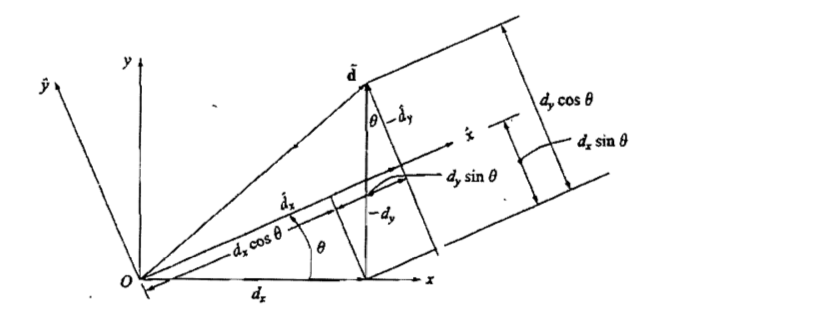
\includegraphics[scale=0.5]{ortho.PNG}
	\caption{Components of vector in x-y and $\hat{x}-\hat{y}$ coordinates} 
	\label{fig:orthof}
\end{figure}
and for Oy or dy, we have
\begin{equation}
	<{t21}\hspace{0.5cm}{t22}>=<{-sin\theta}\hspace{0.5cm}{cos\theta}>
\end{equation}

or unit vectors $\bar{i}$ and $\bar{j}$ can be represented in terms of
unit vectors $\bar{\hat{i}}$ and $\bar{\hat{i}}$.

\begin{equation}
	\bar{\hat{i}} =icos\theta+jsin\theta
\end{equation}

\begin{equation}
	\bar{\hat{j}} =-isin\theta+jcos\theta
\end{equation}

and hence

\begin{equation}
	{t}^2_{11} + {t}^2_{12}=1 
	{t}^2_{21} + {t}^2_{22}=1
\end{equation}

and since these vectors $(\bar{\hat{i}}$ and $\bar{\hat{i}})$ are
orthogonal, by the dot product, we have


\begin{equation}
	<{t}_{11} \bar{i} + {t}_{12} \bar{j}>.<{t}_{21} \bar{i} +
	{t}_{22} \bar{j}>
\end{equation}
or 
\begin{equation}
		{t}_{11}{t}_{21} + {t}_{12} {t}_{22}=0
\end{equation}
or we say \underline{T} is orthogonal and 
therefore $\underline{T}^T\underline{T}=\underline{T}\underline{T}^T=I$ 
and that the transpose is its inverse. That is,

\begin{equation}
	\underline{T}^T=\underline{T}^{-1}
\end{equation}

%----------------------------------------------------------------------------%
%=================1.2.9 Differentiating a Matrix=============================%
%----------------------------------------------------------------------------%

\subsection{Differentiating a Matrix}

A matrix is differentiated by differentiating
 every element in matrix in the conventional 
manner. For example, if

\begin{sagesilent}
	x,y,z=var('x','y','z')
	f=matrix([[x^3,2*x^2,3*x],[2*x^2,x^4,x],[3*x,x,x^5]])
	par=matrix([[x^2,y*x,z*x],[y*x,y^2,y*z],[z*x,y*z,z^2]])
	q=matrix([x,y])
\end{sagesilent}

\begin{equation}
	\underline{a}= \sage{f}
\end{equation}

the derivative $\frac{{\rm d}\underline{a}}{{\rm d}x}$ 
is given by 
\begin{equation} 
	\frac{{\rm d}\underline{a}}{{\rm d}x} = \sage{diff(f,x)}
\end{equation}

Similarly,the partial derivative of a matrix is 

\begin{equation} 
	\frac{\delta\underline{a}}{\delta x}= \frac{\delta \sage{par} 
    }{\delta x} = \sage{diff(par,x)} 
\end{equation}

In structural analysis theory, 
we sometimes differentiate an expression of the form 

\begin{equation}
	U =\sage{q}\left[\begin{array}{rr}a_{11} & a_{12}\\
	a_{21} & a_{22}\\ 
	\end{array}\right]\sage{q.transpose()}
\label{eq:diff}
\end{equation}
where U might represent the strain energy in 
a bar.\eref{eq:diff} is known as a quadratic 
form. By matrix multiplication of \eref{eq:diff}, 
we obtain.

\begin{equation} 
	U = \frac{1}{2}(a_{{11}}x^2 +2a_{{12}}xy + a_{{22}}y^2)
\end{equation}

Differentiating U now yields 
\begin{equation} 
	\frac{\delta U}{\delta x} = a_{{11}}x + a_{{12}}y  
	\frac{\delta U}{\delta y} = a_{{12}}x + a_{{22}}y 
	\label{eq:diff2}
\end{equation} 
\eref{eq:diff2} in matrix form becomes

\begin{equation}
	\left\{\begin{array}{rr} \frac{\delta U}{\delta x} \\
	\frac{\delta U}{\delta y} \\ 
	\end{array}\right\} = \left[\begin{array}{rr}a_{11} & a_{12} \\
	a_{21} & a_{22}\\ 
	\end{array}\right] \sage{q.transpose()}\label{eq:diff3}
\end{equation}

A general form of \eref{eq:diff} is 
\begin{equation} 
	U = \frac{1}{2}\{X\}^T\underline{a}\{X\}
	\label{eq:diff5}
\end{equation}

Then by comparing \eref{eq:diff} and \eref{eq:diff3}, we obtain 
\begin{equation}
	\frac{ \delta U}{\delta x_{i}} = \underline{a}\{X\}
	\label{eq:diff4}
\end{equation}
where $x_{i}$ denotes x and y. Here \eref{eq:diff4} 
depends on matrix \underline{a} in \eref{eq:diff5}being summetric.

%----------------------------------------------------------------------------%
%======================1.2.10 Integrating a Matrix===========================%
%-----------------------------------------------------------------------------%

\subsection{Integrating a Matrix}

Just as in matrix differentiation, to integrate a matrix, we must
integrate every element in the matrix in the conventional manner. For
example, if
$$ \underline{a} = \sage{f}$$
we obtain the integration of $\underline{a}$ as

$$ 
\underline{a}dx = \sage{matrix(3,[c.integrate(x) for row in f for c in row ])
}$$
In our finite element formulation of equations, we often integrate an
expression of the form
\begin{equation}
	\int \underline{X}^T\underline{a}\underline{X} dx dy 
	\label{eq:inte}
\end{equation}

The triple product in \eref{eq:inte} will be symmetric 
if \underline{a} is symmetric. The form 
$\underline{X}^T\underline{a}\underline{X}$ is also called
a quadratic form. For
example, letting
\begin{sagesilent}
	var('x1','x2','x3')
	X=matrix([x1,x2,x3])
\end{sagesilent}

$$\underline{a} = \sage{a} \underline{X}= \sage{X.transpose()}$$
we obtain
\begin{align}
	{X}^T\underline{a}{X} = \sage{X}\sage{a}\sage{X.transpose()} \nonumber\\
	=\sage{X*a*X.transpose()}
\end{align}

which is in quadratic form.

%--------------------------------------------------------------------------%
%===1.3 Cofactor or Adjoint Method to Determine the inverse of a Matrix====%
%-------------------------------------------------------------------------%

\section[Cofactor or Adjoint Method]{Cofactor or Adjoint Method to Determine 
the inverse of a Matrix}

We will now introduce a method for finding the inverse of matrix. This
method is useful for longhand determination of the inverse of smaller
order square matrices (preferably of order 4$\times$4 or less). A
matrix $\underline{a}$ must be square for us to determine its inverse.


We must first define the determinant of a matrix. This concept is
necessary in determining the inverse of a matrix by the cofactor
method. A determinant is a \i{square array of elements expressed by}

\begin{equation}
	|\underline {a}| = |\underline{a_{ij}}|
\end{equation}

where the straight vertical bar, $| |$, on each side of the array denote
the determinant. The resulting determinant of an array will be a
single numerical value when the array is evaluated.

To evaluated the determinant of
$\underline{a}$, we must first determinant the
cofactors of $\underline{a}_{ij}$.
The cofactors of $\underline{a}_{ij}$ are given by

\begin{equation}
	\underline{c}_{ij}=(-1)^{i+j} |\underline{d}|
\end{equation}

where the matrix $\underline{d}$, called the first minor of
 $\underline{a}_{ij}$, is matrix $\underline{a}$ with row 
i and column j deleted. The inverse of matrix
$\underline{a}$ is then given by

\begin{equation}
	\underline{a}^{-1}=\frac{C^{T}}{|\underline{a}|}
	\label{eq:cofinverse}
\end{equation}
where \underline{C} is the cofactor matrix and $|\underline{a}|$ is 
the determine the inverse of a matrix \underline{a} given by 
\begin{sagesilent}
	a=matrix([[-1,3,-2],[2,-4,2],[0,4,1]])
\end{sagesilent}

\begin{equation}
	\underline{a} = \sage{a} 
\end{equation}

Using eq ,we find that the cofactors of matrix \underline{a} are 
\begin{eqnarray}
	  C_{11} = (-1)^{1+1} \left|\begin{array}{rr} -4 &  2 \\4 & 1\\ 
	\end{array}\right| = -12 \nonumber 
	\\C_{12} = (-1)^{1+2} \left|\begin{array}{rr}  2 &  2 \\0 & 1\\ 
	\end{array}\right| =  -2 \nonumber 
	\\C_{13} = (-1)^{1+3} \left|\begin{array}{rr}  2 & -4 \\0 & 4\\ 
	\end{array}\right| =   8 \nonumber 
	\\C_{21} = (-1)^{2+1} \left|\begin{array}{rr}  3 & -2 \\4 & 1\\ 
	\end{array}\right| = -11 \nonumber 
	\\C_{22} = (-1)^{2+2} \left|\begin{array}{rr} -1 & -2 \\0 & 1\\
	 \end{array}\right| =  -1 \nonumber 
	\\C_{23} = (-1)^{2+3} \left|\begin{array}{rr} -1 &  3 \\0 & 4\\ 
	\end{array}\right| =   4 
\label{eq:cofa}
\end{eqnarray} 
 
similarly,

\begin{eqnarray} 
	c_{31} = -2 \nonumber \\ 
	c_{32} = -2 \nonumber \\
	c_{33} = -2 
	\label{eq:cofa2}
\end{eqnarray}

Therefore, from \eref{eq:cofa} and \eref{eq:cofa2} ,we have 
\begin{equation} 
	\underline{c} = \sage{a.adjoint()}
\end{equation}

the determinant of \underline{a} is then 
\begin{equation}
	{|\underline{a}|}=\sum_{j=1}^{n}a_{ij}C_{ij} 
	\text{ with i any row number} 
	(1 < i < n)
	\label{weq:cofa4}
\end{equation}
or
\begin{equation}
	{|\underline{a}|}=\sum_{j=1}^{n}a_{ji}C_{ji} 
	\text{ with i any column number}(1 < i < n) 
\end{equation} 

For instance, if we choose the first of \underline{a} and \underline{c}, 
then i=1 in \eref{weq:cofa4}, and j is summed from 1 to 3 such that
\begin{eqnarray}
	|\underline{a}|=a_{11}C_{11}+a_{12}C_{12}+a_{13}C_{13} \nonumber \\ 
	& = & \sage{a.det()}
\end{eqnarray}
Using the definition of the inverse given by \eref{eq:cofinverse},we have
\begin{equation} 
	\underline{a^{-1}}=\frac{\underline{C}^T}{|\underline{a}|}=\sage{a.inverse()} 
\end{equation}

We can then check that

\begin{equation}
	\underline{a}{a}^{-1}=\sage{matrix.identity(3)}
\end{equation}


The transpose of the cofactor matrix is often defined as the adjoint
matrix; that is,

\begin{equation}
	\ adj\underline{a}=\underline{C}^T 
\end{equation}

Therefore, an alternative equation for the inverse of \underline{a} is


\begin{equation}
	\underline{a}^{-1}=\frac {adj \underline{a}}{|\underline{a}|}
\end{equation}


An important property associated with the determinant of a matrix is
that if the determinant of a matrix is zero ; that is,
$|\underline{a}| =0$ , then the matrix is said to be singular. A
singular matrix does not have an inverse. The stiffness matrices used
in the finite element method are singular until sufficient boundary
conditions (support conditions) are applied. This characteristics of
the stiffness matrix is further discussed in the text.
The inverse of a nonsingular square matrix \underline{a} can be found
by the method of row reduction (sometimes called the Gauss-Jordan
method) by performing identical simultaneous operations on the matrix
\underline{a} becomes an identity matrix and the original identity
matrix becomes the inverse of \underline{a}.

%-------------------------------------------------------------------------%
%==============1.4 Inverse of a Matrix by Row Reduction=====================%
%---------------------------------------------------------------------------%
 
\section[Row Reduction]{Inverse of a Matrix by Row Reduction}\label{last}

A numerical example will best illustrate the procedure. We begin by
converting matrix \underline{a} to an upper triangular form by setting
all elements below the main diagonal equal to zero, starting with the
first column and continuing with succeeding columns. We then proceed
from the last column to the first, setting all elements above the main
diagonal equal to zero.

\begin{sagesilent}
	a=matrix([[2,2,1],[2,1,0],[1,1,1]])
\end{sagesilent}
We will invert the following matrix by row reduction.

\begin{equation}
	\underline{a} = \sage{a}
\end{equation}

To find $\underline{a}^{-1}$, we need to find $\underline{x}$ such that
$\underline{a}\underline{x}=I$, where

\begin{equation}
	\underline{x}=\left[\begin{array}{rrr}
	x_{11} & x_{12} & x_{13} \\
	x_{21} & x_{22} & x_{23} \\
	x_{31} & x_{32} & x_{33} \\
	a_{41} & a_{42} & a_{43}  \\
	\end{array}\right]
\end{equation}

That is,solve
\begin{equation} \sage{a}\underline{x} = \sage{matrix.identity(3)}
\end{equation}
We begin by writing \underline{a} and \underline{I} side by side as

\begin{equation}
	\sage{a.augment(matrix.identity(3))}
	\label{eq:inv1}
\end{equation}

\begin{sagesilent}
	b=matrix([[1,1,1/2],[2,1,0],[1,1,1]])
	b1=matrix([[1/2,0,0],[0,1,0],[0,0,1]])
	c=matrix([[1,1,1/2],[0,-1,-1],[1,1,1]])
	c1=matrix([[1/2,0,0],[-1,1,0],[0,0,1]])
\end{sagesilent}

where the vertical dashed line separates \underline{a} and \underline{I}.
1. Divide the first row of \eref{eq:inv1} by 2.

\begin{equation}
	\sage{b.augment(b1)}
	\label{eq:inv2}
\end{equation}

2.Multiply the first row of \eref{eq:inv2} by -2 and add the result to
the second row.
\begin{equation}
	\sage{c.augment(c1)}
	\label{eq:inv3}
\end{equation}

3. Subtract the first row of \eref{eq:inv3} from the third row.
\begin{equation}
	\sage{matrix([[1,1,1/2,1/2,0,0],[0,-1,-1,-1,1,0],[0,0,1/2,-1/2,0,1]])}
	\label{eq:inv4}
\end{equation}

4. Multiply the second row of \eref{eq:inv4} by -1 and the third row by 2.
\begin{equation}
	\sage{matrix([[1,1,1/2,1/2,0,0],[0,1,1,1,-1,0],[0,0,1,-1,0,2]])}
	\label{eq:inv5}
\end{equation}

5. Subtract the third row of \eref{eq:inv5} from the second row.
\begin{equation}
	\sage{matrix([[1,1,1/2,1/2,0,0],[0,1,0,2,-1,-2],[0,0,1,-1,0,2]])}
	\label{eq:inv6}
\end{equation}

6. Multiply the third row of \eref{eq:inv6} by $-\frac{1}{2}$ and add the
result to the first row.
\begin{equation}
	\sage{matrix([[1,1,0,1,0,-1],[0,1,0,2,-1,-2],[0,0,1,-1,0,2]])}
	\label{eq:inv7}
\end{equation}

7. Subtract the second row of \eref{eq:inv7} from the first row.
\begin{equation} 
	\sage{(matrix.identity(QQ,3)).augment(a.inverse())}
	\label{eq:inv8}
\end{equation}

The replacement of \underline{a} by the inverse matrix is now
complete. The inverse of \underline{a} is then the right side of
\eref{eq:inv8}; that is,
\begin{equation}
	\underline{a}^{-1} = \sage{a.inverse()}
\end{equation}

\end{document}

%----------------------------------------------------------------------------%
%==================================END=======================================%
%--------------------------------------------------------------------------%

